\section{Method}
From the beginning of the design process when each component, 
like part specific functions are briefly defined, the system interactions 
are described as a directed graph.
This allows to do further refinements during the design process, 
by declaring sub-functions, outsource or summarize functionality together.
Tis can be 
Therefore
The individual components therefore have to implement a certain interface, 
which allows to set the inputs and update the outputs accordingly.
\begin{figure}[h]
    \centering
    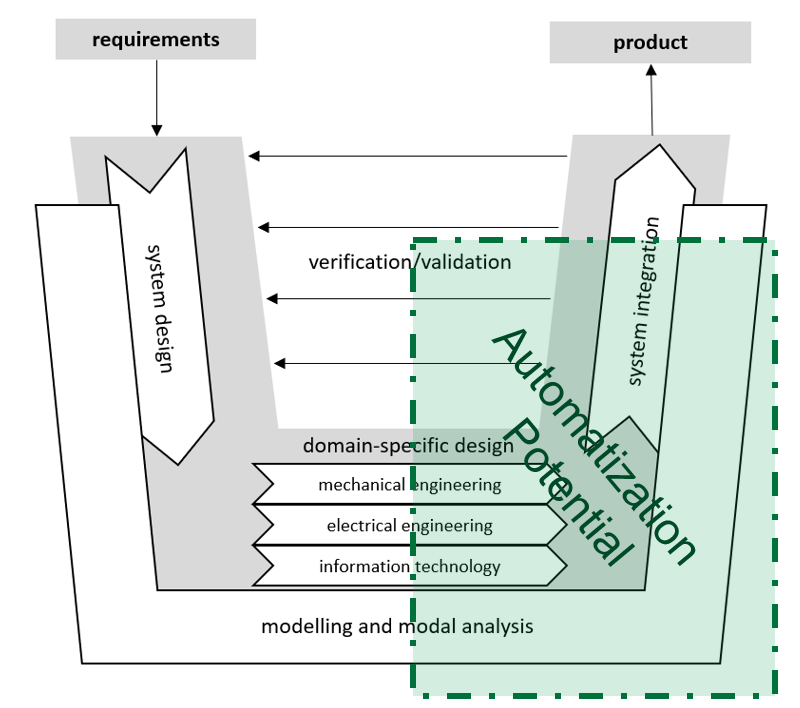
\includegraphics[scale=0.5]{pics/VDI_2206.PNG}
    \caption{\label{pic:VDI2206} "General approach for development and construction (VDI 2221)." \cite{Jansch2006THEDO}}
\end{figure}\\
Using a directed graph method to represent each process Each step in a workflow can be represented as blackbox with a certain input and output (fig. \ref{pic:process-single}).
Due to simplicity the inputs and outputs have values that consists of a list of numbers. 
This values may be connected to other steps in the workflow resulting in different dependencies.
\begin{figure}[h]
    \centering
    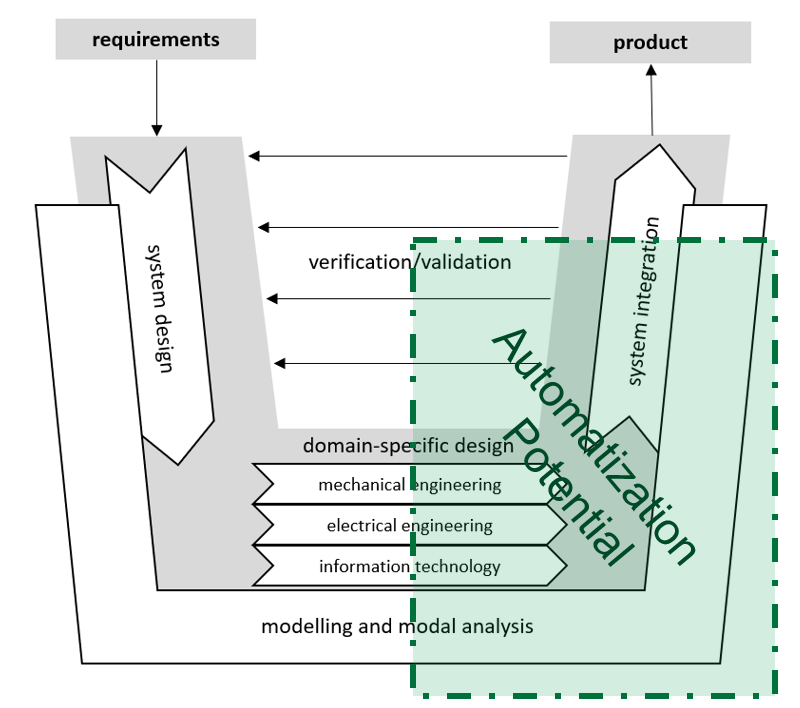
\includegraphics[scale=0.5]{pics/VDI_2206.PNG}
    \caption{\label{pic:VDI2206} "General approach for development and construction (VDI 2221)." \cite{Jansch2006THEDO}}
\end{figure}\\
test
\begin{algorithm}[ht]
    \SetAlgoLined
    \KwIn{list of porcesses}
    \KwOut{sortet list of processes}
    use bubble sort to sort the list\; 
    \Fn{\FBSort{Process A, Process B}}{
        \eIf{A.InputConnections == B.InputConnections}{
            \eIf{A.Time == B.Time}{
                \eIf{A.InputConnections-A.InputChanges == B.InputConnections-B.InputChanges}{
                    \eIf{A.InputChanges == B.InputChanges}{
                        \Return{A.OutputConnections $<$ B.OutputConnections}
                    }{
                        \Return{A.InputChanges $>$ B.InputChanges}
                    }
                }{
                    \Return{A.InputConnections-A.InputChanges $<$ B.InputConnections-B.InputChanges}
                }
            }{
                \Return{A.Time $<$ B.Time}
            }
        }{
            \Return{A.InputConnections $<$ B.InputConnections}
        }
    }
    \textbf{end}
\caption{\label{code:sort-process}Sort-Algorithm}
\end{algorithm}
text
\begin{algorithm}[bt]
    \KwIn{List of Processes\\
    Priority $\in$ ["manual", "dynamic", "time"]}
    \KwOut{Updated and converged processes}
    sort(List of Processes)\;
    \textbf{set} GState to "changed"\;
    \textbf{set} StartPos to 0\;
    \While{GState = "changed"}{
        \textbf{set} GState to "unchanged"\;
        \For{i = StartPos to sizeof(List of Processes)}{
            \textbf{set} CurrProcess as ith Element of List of Processes
            \textbf{set} GState to "unchanged"\;
            \textbf{set} STime to currentTime()\;
            \textbf{set} PState to CurrProcess.update()\;
            \textbf{set} ETime to currentTime()\;
            \textbf{set} $\Delta$Time to ETime - STime\;
            \If{Priority equals "time"}{
                CurrProcess.Time = round($\log_{10}${$\Delta$Time})\;
            }
            \If{PState equals "changed"}{
                \textbf{set} GState to "changed"\;
            }
            \If{CurrProcess.Inputs equals 0 \emph{\textbf{and}} Priority not "manuel"}{
                \textbf{set} StartPos to i\;
            }
            \If{Priority equals "dynamic" \emph{\textbf{or}} Priority equals "time"}{
                \textbf{set} List of FProcesses as List of Processes starting from CurrProcess\;
                \ForEach{FurtherProcess in  List of FProcesses}{
                    FurtherProcess.InputChanges.update()\;
                }
                sort(List of FProcesses)\;
            }
            increase i by one\;
       }
    }
\caption{\label{code:update-standard-processor}Update-Algorithm of the standard processor}
\end{algorithm}\\
Test
Test
test
\begin{figure}[h]
    \centering
    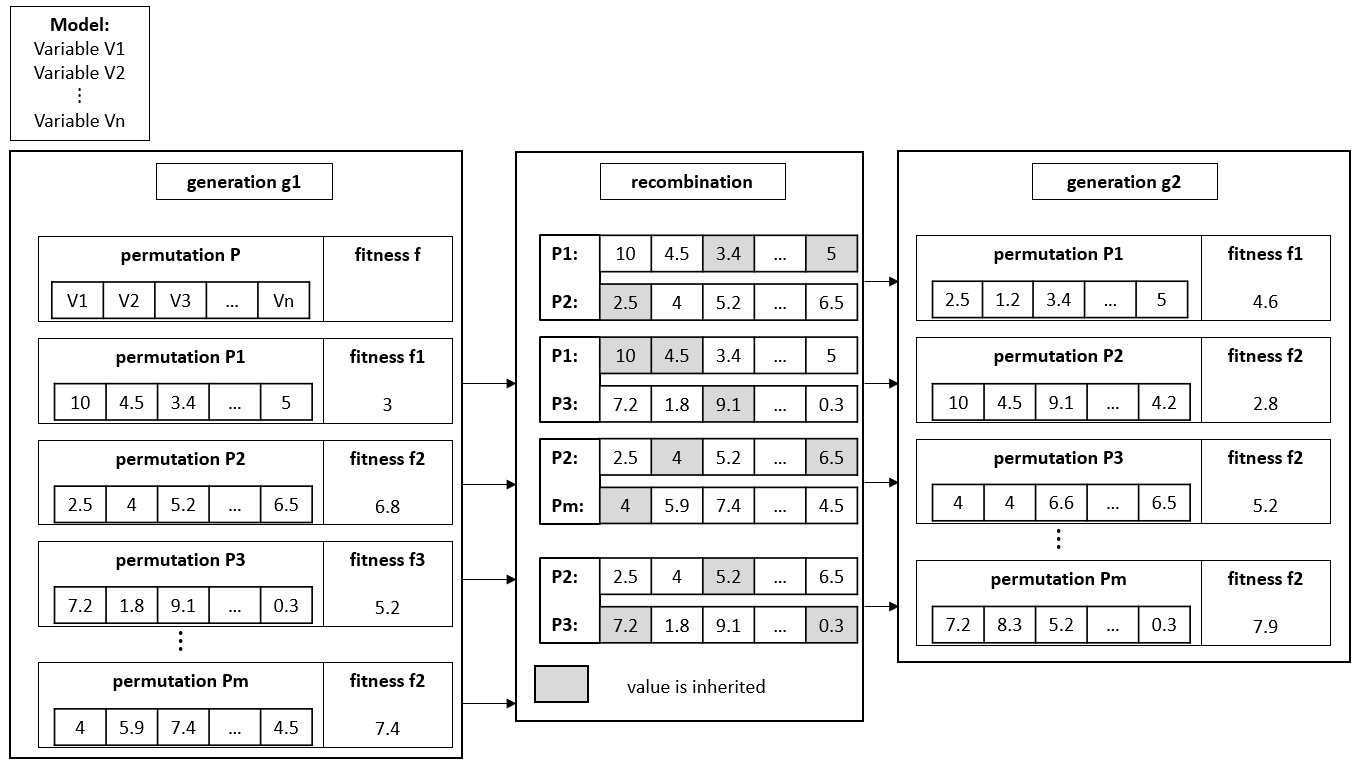
\includegraphics[scale=0.5]{pics/evol_alg.PNG}
    \caption{\label{pic:evol_alg} "General approach for development and construction (VDI 2221)." \cite{Jansch2006THEDO}}
\end{figure}\\
test
